% Copyright 2023 Gerald Brandi Cainicela Aquino. 
% Todos los derechos reservados. 
% Contacto: gerald.cainicela.a@gmail.com

% Copyright 2023 Gerald Brandi Cainicela Aquino. 
% Todos los derechos reservados. 
% Contacto: gerald.cainicela.a@gmail.com

\documentclass[a4paper,10pt,sans]{article} % Fornato, estilo y el tipo de documento
\usepackage[utf8]{inputenc} % Permite el uso de caracteres Unicode en el código fuente del documento.
\usepackage[T1]{fontenc} % Configura la codificación de la fuente para admitir caracteres acentuados y especiales.
\usepackage[spanish]{babel} % Adapta el documento para su uso en español, ajustando nombres y etiquetas automáticamente.
\usepackage[top=1in, left=1in, right=1in, bottom=1in]{geometry} % Ajusta los márgenes del documento a 1 pulgada en cada lado.
\usepackage{academicons} % Proporciona acceso a iconos específicos para el ámbito académico.
\usepackage{ebgaramond} % Carga la fuente EB Garamond en el documento.
\usepackage{fontawesome5} % Permite la inclusión de iconos de la popular fuente de iconos Font Awesome.
\usepackage{hyperref} % Permite la creación de enlaces y referencias cruzadas en el documento.
\usepackage{multicol} % Facilita la creación de columnas múltiples en el documento.
\usepackage{pagecolor} % Facilita el cambio de color de la página en el documento.
\usepackage{ragged2e} % Proporciona comandos adicionales para justificar el texto y controlar la alineación en el documento.
\usepackage{sectsty} % Facilita el cambio de estilos de secciones en el documento.
\usepackage{titlesec} % Ofrece herramientas para personalizar y cambiar el formato de los títulos de las secciones.
\usepackage{xcolor} % Proporciona funcionalidades adicionales para el color en el documento.
\usepackage{xstring} % Proporciona manipulación avanzada de cadenas de texto.
\usepackage{graphicx} % Permite la inclusión de gráficos en el documento.
\usepackage{changepage} % Facilita los ajustes personalizados de diseño de página.
\usepackage{ifthen} % Proporciona comandos condicionales avanzados.
\usepackage{etoolbox} % Proporciona herramientas para la manipulación de comandos y entornos LaTeX.


 
%---cambiar acorde a tus datos
\newcommand{\myName}{Aqui va el Nombre}
\newcommand{\myDegree}{Lo que estudioo estudié}
\newcommand{\perfil}{asset/img/perfil.png} % en aqui va el perfil, debe ir a ese directorio
%---
% Copyright 2023 Gerald Brandi Cainicela Aquino. 
% Todos los derechos reservados. 
% Contacto: gerald.cainicela.a@gmail.com


% Configuración de hipervínculos
\hypersetup{
	colorlinks=true,
	linkcolor=blue,
	filecolor=magenta,      
	urlcolor=blue,
	pdftitle={\myName},
	pdfpagemode=FullScreen,
}

% Definición de un color para las secciones
\definecolor{colorSection}{HTML}{2C7ECB}

% Configuración de la fuente y el estilo de las secciones utilizando el paquete sectsty
\sectionfont{\color{colorSection}\large\bfseries}

% Configuración de la apariencia de las secciones con el paquete titlesec
\titleformat{\section} 
{\color{colorSection}\Large\bfseries}
{}
{0em}
{}[\color{colorSection}\titlerule]


\newcommand{\siPerfil}{true}
\newcommand{\noPerfil}{false}

\newcommand{\miTitulo}[2]{%
	\ifthenelse{\equal{#2}{\siPerfil}}{%
		\begin{minipage}{0.76\textwidth}
			\begin{flushleft} 
				\textbf{\LARGE \MakeUppercase{\myName}}\\
				\vspace{0.2cm}
				\Large\  \textbf{\myDegree}
			\end{flushleft}
			\vspace{0.2cm}
			#1
		\end{minipage}%
		\begin{minipage}{0.4\textwidth}
			\begin{adjustwidth}{0.65cm}{}
			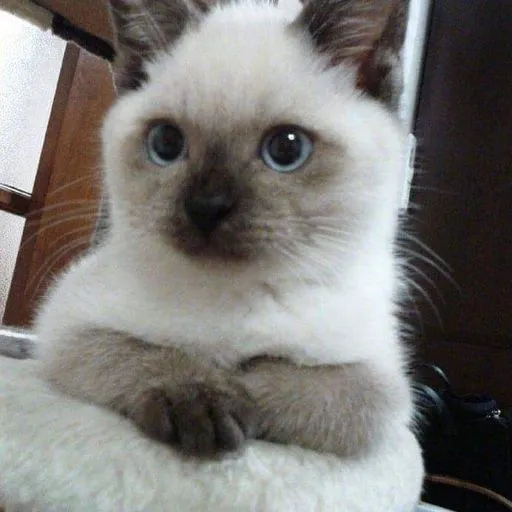
\includegraphics[width=0.5\linewidth]{\perfil}
			\end{adjustwidth}
		\end{minipage}%
	}{%
		\ifthenelse{\equal{#2}{\noPerfil}}{%
			\begin{flushleft} 
				\textbf{\LARGE \MakeUppercase{\myName}}\\
				\vspace{0.2cm}
				\Large\  \textbf{\myDegree}
			\end{flushleft}
			\vspace{0.2cm}
			#1
		}{}%
	}%
}


% Definición de un comando para la sección de datos personales
\newcommand{\datosPersonalesSec}[1]{%
	\section*{Datos Personales}
	\begin{tabular}{p{3cm}p{12cm}}
		#1
	\end{tabular}
}

% Definición de un comando para la sección de formación académica
\newcommand{\formacionAcademica}[5]{%
	\begin{tabular}{p{11cm}p{10cm}}
		\textbf{#1 } &  \\
		\quad\textbf{  #2 } & #4- #5 \\
		\qquad\textit{#3 } &  \\
	\end{tabular}
}

 

% Definición de la función datosPersonales que toma tres argumentos y verifica si el segundo y tercer argumento son direcciones de correo electrónico o URL antes de formatearlos
\newcommand{\datosPersonales}[3]{%
	% Imprime el texto en negrita seguido del primer argumento y un separador
	\textbf{#1:}  &
	% Verifica si el segundo argumento contiene un símbolo de correo electrónico
	\IfSubStr{#2}{@}{\href{mailto:#2}{#2}}{%
		% Verifica si el segundo argumento contiene '.com' o '.pe'
		\IfSubStr{#2}{.com}{\href{#2}{\url{#2}}}{%
			\IfSubStr{#2}{.pe}{\href{#2}{\url{#2}}}{#2}%
		}
	} \\
	% Verifica si el tercer argumento está vacío, si no, verifica si es un correo electrónico o una URL y lo formatea como un enlace
	\ifx\empty#3\else & 
	\IfSubStr{#3}{@}{\href{mailto:#3}{#3}}{%
		\IfSubStr{#3}{.com}{\href{#3}{\url{#3}}}{%
			\IfSubStr{#3}{.pe}{\href{#3}{\url{#3}}}{#3}%
		}
	} \\ 
	\fi
}

\newcommand{\noObjetivo}{

}

\newlength{\mySpaceTask}
\setlength{\mySpaceTask}{0.3889em} % denota 7/18, es decir \:\,  0.3889em 4+3/18
\newcommand{\task}[1]{%
	%\hspace{\mySpaceTask} 
	
	\begin{minipage}{0.2cm} 
		\:
	\end{minipage}
	\begin{minipage}{\mySpaceTask} 
			\textbullet
	\end{minipage}
	\begin{minipage}{\dimexpr\textwidth-\mySpaceTask-2cm\relax}
	 #1
	\end{minipage}

}

\newcommand{\taskV}[1]{%
	%\hspace{\mySpaceTask} 
	
	\begin{minipage}{0.2cm} 
		\:
	\end{minipage}
	\begin{minipage}{\mySpaceTask} 
		\,
	\end{minipage}
	\begin{minipage}{\dimexpr\textwidth-\mySpaceTask-2cm\relax}
		#1
	\end{minipage}
	
}


	%\:=4/18
	%\, =3/18
\newcommand{\experienciaProyecto}[6]{%
	\begin{tabular}{p{12.4cm}p{3cm}}
		\textbf{#1} &\\
		#2 & #3 - \\
		\ifx#5\noObjetivo
		\else
		\textbf{Objetivo: } #5 & #4\\
		\fi
	\end{tabular} 
	
	\medskip
	#6
	\vspace{0.5cm}
}
\newcommand{\experienciaProyectoV}[6]{%
	\begin{tabular}{p{9.6cm}p{4.4cm}}
		\textbf{#1} &\\
		\textbf{#2} & \hfill #3 - #4
	\end{tabular}
	
	\ifx#5\noObjetivo
	\else
	\begin{tabular}{p{15.4cm}}
		\textbf{Objetivo: } #5
	\end{tabular} 
	\fi
	
	\smallskip
	#6
	\vspace{0.5cm}
}
 
 
\newcommand{\experienciaLaboral}[5]{%
	\begin{tabular}{p{9.6cm}p{4.4cm}}
		\textbf{#1} &\\
		\textbf{#2} & \hfill #3 - #4
	\end{tabular}
	
	\smallskip
	#5
	\vspace{0.5cm}
}



\newcommand{\voluntariadoAcademico}[5]{%
	\begin{tabular}{p{9.6cm}p{4.4cm}}
		\textbf{#1} &\\
		\textbf{#2} & \hfill #3 - #4
	\end{tabular}
	
	\smallskip
	\,\: #5
	\vspace{0.2cm}
	
}



\newcommand{\competenciasDigitales}[1]{%
	\begin{tabular}{p{5cm}p{10cm}}
		#1
	\end{tabular}
}
\newcommand{\habilidadesPersonales}[1]{%
	\begin{tabular}{p{5cm}p{10cm}}
		#1
	\end{tabular}
}
\newcommand{\idiomas}[1]{%
	\begin{tabular}{p{4cm}p{12cm}}
		#1
	\end{tabular}
}
\newcommand{\taskC}[2]{% 
	\textbullet	\ #1: & #2\\
}
\begin{document}
	 
	%\justify %justificar 
	%\pagecolor{gray!5} % Cambia el color de fondo aquí

	\miTitulo{
		Soy una persona apasionada por la innovación y la tecnología, con sólida formación académica y habilidades en resolución de problemas, trabajo en equipo y liderazgo. Soy proactivo y adaptable a nuevos desafíos. Busco contribuir al desarrollo tecnológico y crecer profesionalmente en una empresa líder en ingeniería.
		}{true} % 	true: si tiene alguna foto
				%	false: no tienes ninguna foto

	\datosPersonalesSec{
		\datosPersonales{Correo(s)}{correo1@example.com}{correo2@example.com}
		\datosPersonales{N° Celular(es)}{987654321}{987654321}
		\datosPersonales{LinkedIn}{www.linkedin.com/in/gerald-cainicela}{}
		\datosPersonales{GitHub}{https://github.com/asdcainicela}{}
	}

	\section*{Formación Académica}
	
		\formacionAcademica
		{Universidad Nacional de Ingeniería}
		{Egresado en \myDegree}
		{Quinto Superior}
		{03/2019}{7/2023} %fecha de inicio y fin respectivamente

	\section*{Experiencia Laboral}
		\experienciaLaboral
		{Mining Mechatronick}
		{Ingeniero de Control y Automatización}
		{01/08/2023}{Actualidad}
		{
			\task{Encargado del desarrollo de proyectos de automatización para maquinaria utilizada en minería subterránea, brindando soluciones innovadoras y eficientes para optimizar los procesos en este entorno exigente. }
			\task{Experto en programación de HMI's, controladores y gateways IoT mediante el uso de CoDeSys 3.5, proporcionando interfaces amigables y funcionales para nuestros clientes y garantizando la integración de los dispositivos en nuestros proyectos. }
			\task{Proveer un soporte técnico especializado para los dispositivos de automatización ofrecidos por la empresa, asegurando un acompañamiento integral a nuestros clientes durante todas las etapas de implementación y mantenimiento, y garantizando su satisfacción con nuestros productos y servicios.}
		}

		\experienciaLaboral{Nombre de la Empresa}
		{Rol en la empresa}
		{Inicio}{Final}
		{
			\task{Tareas o actividades que desarrollabas en la empresa}
			\task{Tareas o actividades que desarrollabas en la empresa}
		}


	\section*{Experiencia en Proyectos}

		\experienciaProyectoV
		{Organización}
		{Rol o función}
		{inicio}{final}
		{Objetivo} % si no tiene ningún objetivo, debe poner \noObjetivo
		{
			\task{Tarea o actividad 1} 
			\task{Tarea o actividad 1} 
			\task{Tarea o actividad 1} 
		}

		\experienciaProyectoV{Wayta Wayra, UNI, UNIFIM, CEDIME}
		{Director de Proyecto}
		{04/07/2023}{Actualidad}
		{Diseño y Desarrollo de Aerogeneradores Savonius para la Recarga de Bicicletas y Vehículos Eléctricos, así como para la Mejora de la Iluminación Pública en las Avenidas Principales de Lima. }
		{
			\task{Participación en el diseño y construcción de la tarjeta electrónica CubeSat}
			\task{Utilización de herramientas como CAE (Computer-Aided Engineering) y CAD (Computer-Aided Design) con SolidWorks y Ansys. }
			\task{Coordinación con los equipos multidisciplinarios para asegurar la optimización del rendimiento y la eficiencia energética. }
			\task{Colaboración y comunicación efectiva con los equipos internos y stakeholders para cumplir con los objetivos planteados.}
		} 
		
	
	\section*{Voluntariado Académico}
		\voluntariadoAcademico{Organización}{Función o rol}{inicio}{fin}
		{que hiciste, una breve descripción}
		\voluntariadoAcademico{UNI - RA OPT-FIM }{Tutor}{03/2023}{07/2023}
		{Elaboración de material de estudio y dictado de clases de Cálculo Integral para estudiantes en riesgo académico.}

	
	\section*{Competencias Digitales}
		\competenciasDigitales{
			\taskC{Rama principal}{Secundarias}
			\taskC{ Herramientas de Microsoft Office}{Excel, Power BI, Power Query, Word, PowerPoint, Microsoft Teams}
			\taskC{Lenguajes de Programación}{Matlab, C, C++, Python, Java }
			\taskC{Composición de Documentos}{\LaTeX}
		}
	

	
	\section*{Habilidades Personales}
		\habilidadesPersonales{
			\taskC{Adaptabilidad:}{ Flexibilidad para enfrentar desafíos y ajustarse a cambios.}
			\taskC{Comunicación efectiva}{Capacidad para transmitir ideas y conceptos de manera clara y concisa.} 
			\taskC{Innovación y Creatividad:}{ Capacidad para generar ideas originales y soluciones creativas.} 
			\taskC{Liderazgo y Capacidad de Gestión:}{Experiencia en guiar equipos hacia el logro de objetivos.} 
			\taskC{ Relaciones Interpersonales:}{ Competencia en establecer y mantener relaciones efectivas.} 
			\taskC{Organización:}{ Habilidad para planificar y coordinar tareas de manera efectiva.}
			\taskC{Pensamiento Analítico:}{ Capacidad para descomponer problemas y tomar decisiones informadas. }
			\taskC{Resiliencia:}{antener calma y productividad bajo presión. }
			\taskC{Resolución de Problemas:}{Habilidad para analizar situaciones complejas y generar soluciones efectivas. }
			\taskC{Toma de Decisiones: }{Capacidad para evaluar opciones y tomar decisiones informadas. }
			\taskC{Trabajo Bajo Presión: }{Habilidad para mantener el enfoque y la eficiencia en situaciones desafiantes. }
			\taskC{Trabajo en Equipo: }{Colaborar en equipos multidisciplinarios para lograr objetivos comunes. }
		}
 
	\section*{Idiomas}
		\idiomas{
			\taskC{Idioma}{ Nivel}
			\taskC{Español}{ Nativo }
			\taskC{Inglés}{ Intermedio }
		}
\end{document}